% Use only LaTeX2e, calling the article.cls class and 12-point type.

\documentclass[12pt]{article}

% Users of the {thebibliography} environment or BibTeX should use the
% scicite.sty package, downloadable from *Science* at
% www.sciencemag.org/about/authors/prep/TeX_help/ .
% This package should properly format in-text
% reference calls and reference-list numbers.

% Use times if you have the font installed; otherwise, comment out the
% following line.

\usepackage{times,amsmath}
\usepackage{empheq}
\usepackage[theorems,skins]{tcolorbox} % for nice boxed eqs
\newtcolorbox{mymathbox}[1][]{colback=white, sharp corners, #1}

% for figs
\usepackage{graphicx}
\usepackage{float}

% The preamble here sets up a lot of new/revised commands and
% environments.  It's annoying, but please do *not* try to strip these
% out into a separate .sty file (which could lead to the loss of some
% information when we convert the file to other formats).  Instead, keep
% them in the preamble of your main LaTeX source file.


% The following parameters seem to provide a reasonable page setup.

\topmargin 0.0cm
\oddsidemargin 0.2cm
\textwidth 16cm
\textheight 21cm
\footskip 1.0cm

%The next command sets up an environment for the abstract to your paper.

\newenvironment{sciabstract}{%
\begin{quote} \bf}
{\end{quote}}


% If your reference list includes text notes as well as references,
% include the following line; otherwise, comment it out.

\renewcommand\refname{References and Notes}

% The following lines set up an environment for the last note in the
% reference list, which commonly includes acknowledgments of funding,
% help, etc.  It's intended for users of BibTeX or the {thebibliography}
% environment.  Users who are hand-coding their references at the end
% using a list environment such as {enumerate} can simply add another
% item at the end, and it will be numbered automatically.

\newcounter{lastnote}
\newenvironment{scilastnote}{%
\setcounter{lastnote}{\value{enumiv}}%
\addtocounter{lastnote}{+1}%
\begin{list}%
{\arabic{lastnote}.}
{\setlength{\leftmargin}{.22in}}
{\setlength{\labelsep}{.5em}}}
{\end{list}}

\renewcommand{\baselinestretch}{1.3} % 1.5 line spacing
\setlength{\parindent}{4em}
\setlength{\parskip}{1em}

% Include your paper's title here

\title{AM205 Project - Traffic Flow Modelling\\
\Large{Microscopic Models of Traffic, Comparing the Intelligent Driver Model (with Adaptive Cruise Control) with the Human Driver Model}}


% Place the author information here.  Please hand-code the contact
% information and notecalls; do *not* use \footnote commands.  Let the
% author contact information appear immediately below the author names
% as shown.  We would also prefer that you don't change the type-size
% settings shown here.

\author
{Anna Hilgard, Sam Daulton and Nicholas Hoernle}

% Include the date command, but leave its argument blank.

\date{}



%%%%%%%%%%%%%%%%% END OF PREAMBLE %%%%%%%%%%%%%%%%



\begin{document}


% Make the title.

\maketitle

\section{Introduction}

\paragraph{}
The modeling of traffic at traffic lights, on highways, in dense traffic streams, with varying situations etc can often present a problem that is too complicated to solve analytically. This is mainly due to the inherent random movements of cars, the number of individually moving cars and the many and varying scenarios that can be analyzed.
In this project, we present two main models, the `Intelligent Driver Model' and the `Human Driver Model' and numerically simulate a number of test cases allowing us to study the underlying dynamics of this system. We focus on modeling the cars using a differential setting where one car's motion is dependent on the car that is in front of it (and sometimes dependent on multiple cars in front of it). We will then extend the scope of this analysis and introduce a number of varying factors into the model to analyze the motion of cars along a straight road, analyze the cars along a circular track and finally include a blend of the intelligent driving cars (comparable to automated cruise control autonomous cars) and cars with the human controlled vehicles. These autonomous cars have more precise, and faster reacting velocity controllers and the inclusion of vehicles such as these in the model is expected to smooth the flow of traffic and ultimately increase the density of traffic flow.

\paragraph{}There are generally two ways to model traffic: from a microscopic and from a macroscopic perspective \cite[Chapter~34]{microscopic_modelling}. In the macroscopic perspective, traffic is viewed as a fluid or gas with a given maximum density moving according to the laws of conservation of mass. Because we'd like to interweave different models for specific cars, these models would be difficult to blend in a way that is easily interpretable.

\section{Microscopic Perspective of Single Lane Traffic Interactions}
\paragraph{} In the microscopic perspective, individual cars are modeled as particles that move according to a relationship with the particle(s) in front of them.  Time-continuous microscopic models, commonly referred to as car-following models, model the characteristics of individual vehicles such as acceleration, velocity, position using a systems of coupled ordinary differential equations (ODEs).  Car-following models are constained by assumptions that mimic realistic driving behavior such as a vehicle wants to maintain a safe driving gap between itself and vehicle in front of it (commonly called the \textit{leading vehicle}), a vehicle has a certain desired velocity, or there is a maximum comfortable acceleration \cite[chapter~10]{treiber_kesting_2013}. In the section, we consider a few variations of the Intelligent Driver Model (IDM), as well as Human Driver Model (HDM).  
%We chose the IDM over other car-following models such as Gipps Model because the IDM has direct extensions to modeling human driving behavior using the HDM.
We chose the IDM over other car-following models such as the Gipps Model or Newell's due to the oversimplification of some acceleration assumptions that the alternative models make\cite[chapter~11]{treiber_kesting_2013}. The result is that the IDM provides the simplest implementation of plausible driving characteristics.
\subsection{Intelligent Driver Models}
In this section, we model streams of semi-autonomous vehicles that display the following driving characteristics:
\begin{itemize}
  \item No estimation errors: each vehicle is aware of its own speed, the gap between itself the car in front of it, and the speed of the car in front of it.
  \item Zero response time: there is no delay between observing a stimulus (i.e. change in gap between itself and vehicle ahead of it or change the vehicle ahead's speed) and responding to it.
  \item Constant attention: the vehicle is constantly looking for changes in speed or gap
  \item Each vehicle is only aware of itself and the vehicle directly in front of it.  I.e. it does not account for changes in speed or gap of a vehicle two cars ahead of it.
  \item Each vehicle is not aware of vehicles behind it or in other lanes
  \item Vehicles are not aware other indicators such as brake lights, horns, headlight flashes, etc.
\end{itemize}
\subsubsection{Intelligent Driver Model (IDM)}
\begin{figure}
  \centering
  \fbox{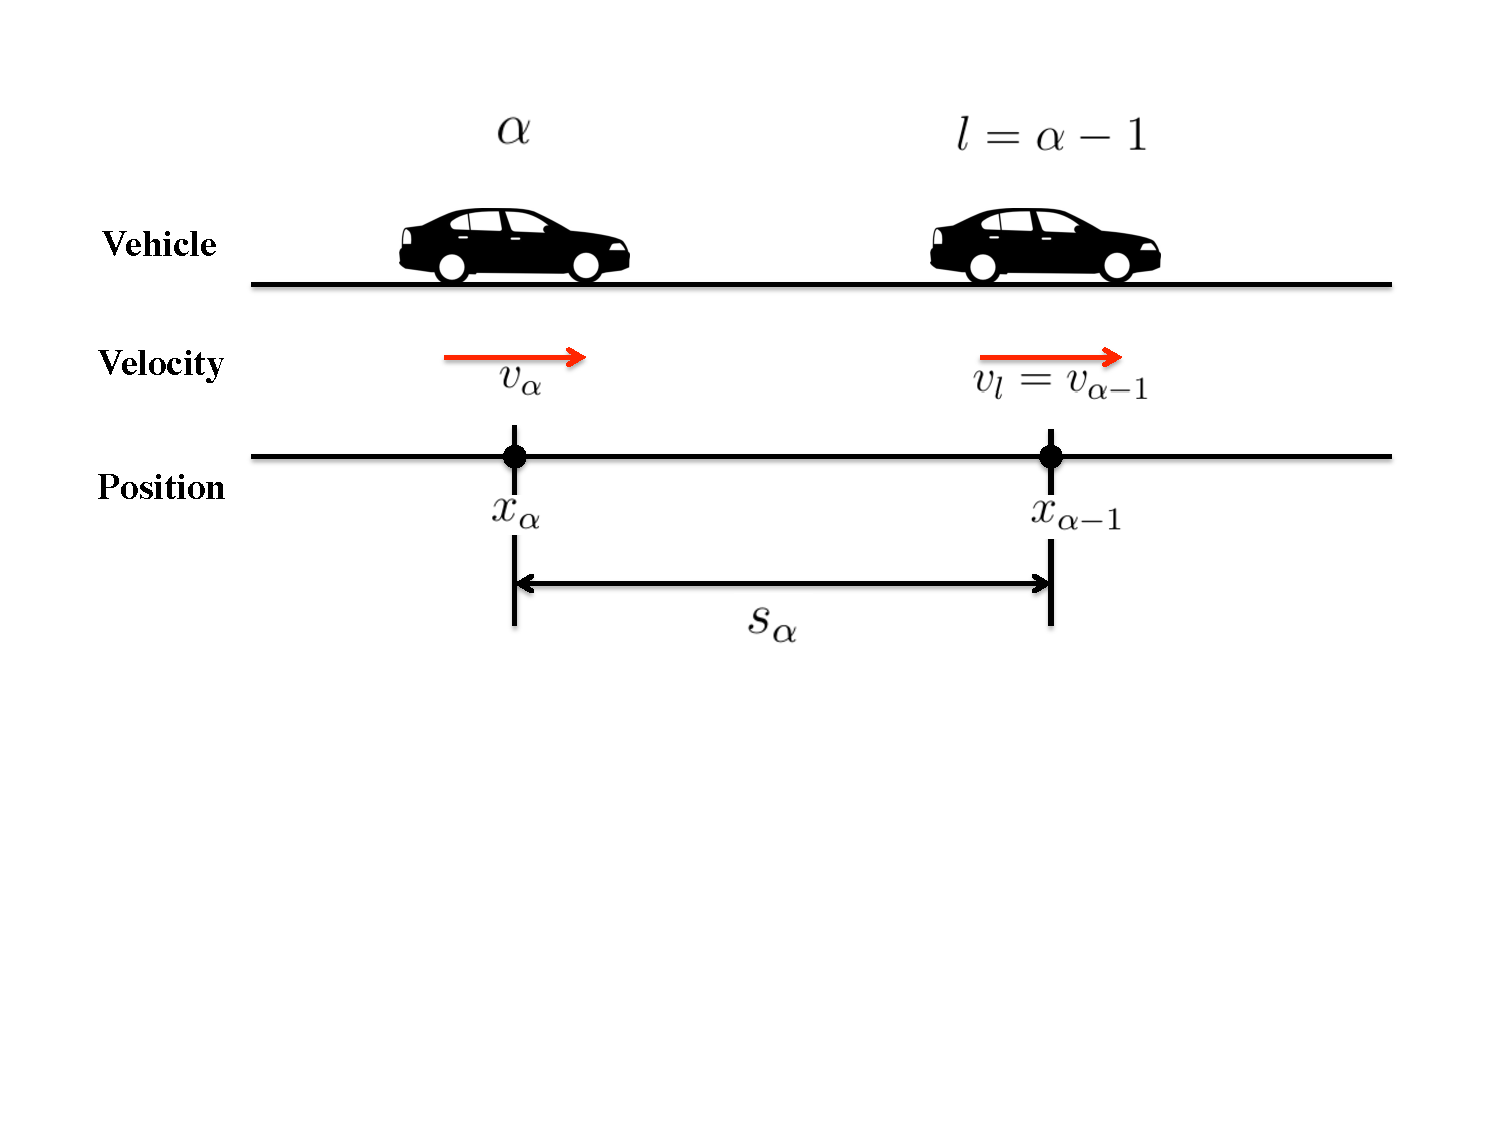
\includegraphics[width=0.95\textwidth]{../figures/system_ppt_fig}}
  \caption{Snapshot of two cars in a system modeled using a car-following model.  The leading car with respect to vehicle $\alpha$  is referred to as vehicle $l=\alpha-1$.  Note that vehicles are represented as particles, and therefore, the vehicles themselves have negligible length.}
\end{figure}
\paragraph{}
The IDM is a simple, accident-free model that can model traffic systems under all realistic traffic conditions.  The acceleration function, shown in Eq (1), of a particular vehicle $\alpha$ is a function the current gap between itself and the leading vehicle ($s_\alpha$), the desired speed $v_0$, and the speed of the vehicle leading vehicle $v_l$.  

\begin{mymathbox}[title=IDM Parameters, colframe=blue!30!black]
  \begin{itemize}
    \item $a$: maximum acceleration
    \item $b$: maximum comfortable deceleration
    \item $s_0$: minimum bumper-to-bumper gap (between vehicle and leading vehicle)
    \item $v_0$: desired speed
    \item $T$: minimum time gap (between vehicle and leading vehicle)
    \item $\delta$: acceleration exponent
  \end{itemize}
\end{mymathbox}

\begin{mymathbox}[ams gather, title=IDM Governing Equations, colframe=blue!30!black]
  \begin{align}
  \dot{v}_\alpha &= a \left[1 - \left(\frac{v_\alpha}{v_0}\right)^{\delta} - \left(\frac{s^*(v_\alpha,\Delta v_\alpha)}{s_\alpha}\right)^{2}\right]\\
  s_\alpha &= x_{\alpha-1}-x_\alpha=x_{l}-x_\alpha\\
  \Delta v_\alpha &=v_\alpha-v_{\alpha-1}=v_\alpha-v_l\\
  s^*(v_\alpha, \Delta v_\alpha) &= s_0 + \max\left(0, v_\alpha T + \frac{v_\alpha \Delta v_\alpha}{2 \sqrt{ab}} \right)
  \end{align}
\end{mymathbox}
\paragraph{}
The first term in Eq (1) is the \textit{free acceleration}\---the acceleration that a vehicle would take if on an open road, without considerations of desired speed or gap.  The second term in Eq (1) is the effect on the acceleration of the vehicle approaching its desired speed.  The third term in Eq(1) is the effect on the acceleration of relative difference between the desired gap distance $s^*(v_\alpha,\Delta v_\alpha)$ and the current gap distance.  The desired gap distance given by Eq (4) the sum of two terms the steady state desired safe distance $s_0+v_\alpha T$ and a dynamical term $\frac{v_\alpha \Delta v_\alpha}{2 \sqrt{ab}}$ representing the intelligent vehicle's braking strategy \cite{intelligent_driver_model}.

\subsubsection{Improved Intelligent Driver Model (IIDM)}
\paragraph{}
The Improved Intelligent Driver Model is an IDM model with an improved acceleration function that aims to correct two unrealistic qualities of the IDM when a vehicle is near the desired speed:
\begin{enumerate}
  \item 
  If a vehicle exceeds the desired speed, the IDM acceleration function will return a very large negative acceleration.  This is unrealistic since drivers on a highway tend to oscillate around their desired speed.  
  \item
  If a vehicle is close to the desired speed, the desired gap $s^*(v_\alpha,\Delta v_\alpha)$ becomes much greater than $s_0 + v_\alpha T$.  This causes the gaps between vehicles to be unrealistically large and can preclude vehicles from reaching the desired velocities.
\end{enumerate}
\begin{mymathbox}[ams gather, title=IIDM Governing Functions, colframe=blue!30!black]
  \begin{align}
  \frac{dv_\alpha}{dt}\Bigr|_{v_\alpha\le v_0}&= 
  \begin{cases}
    a (1-z_\alpha^2) & z_\alpha \ge 1\\
   a_{\text{free},\alpha}(1 - z_\alpha^{(2a)/a_{\text{free},\alpha}})& \text{otherwise}
  \end{cases}
  \\
  \frac{dv_\alpha}{dt}\Bigr|_{v_\alpha> v_0}&= 
  \begin{cases}
    a_{\text{free},\alpha} + a (1-z_\alpha^2) & z_\alpha \ge 1\\
    a_{\text{free},\alpha} & \text{otherwise}
  \end{cases}\\
  a_{\text{free},\alpha}(v_\alpha)&= \begin{cases}
  a \left[ 1 - (\frac{v_\alpha}{v_0})^\delta \right] & v_\alpha \le v_0\\
  -b \left[ 1 - (\frac{v_0}{v_\alpha})^{a\delta/b} \right] & v_\alpha > v_0
  \end{cases}\\
  z_\alpha&= \frac{s^*(v_\alpha, \Delta v_\alpha)}{s_\alpha}
  \end{align}
\end{mymathbox}
\paragraph{}
The IIDM governing equations seek to improve the unrealistic qualities of the IDM model. Eq (8) is the free acceleration equation, which limits the deceleration's magnitude when $v_\alpha>v_0$ to be at most b. To improve the acceleration function near the desired speed, we use $z_\alpha$ to indicate whether the desired gap distance is greater than the current gap distance or not.  When $v_\alpha < v_0$, the IIDM's acceleration function (Eq (5) and Eq (6)) ensures that the actual gap is no larger than the minimum safe gap $s_\alpha = s_0+vT$.  To maintain the intelligent and comfortable brake method of the IDM, the improved acceleration function only changes when the actual gap is near the desired gap or when the actual velocity is greater than the desired velocity.
\subsubsection{Adaptive Cruise Control Model (ACC)}
\paragraph{}
The ACC is an improvement on the IIDM model that is designed so that a vehicle can handle is discontinuous changes in the gap between itself and the leading vehicle or discontinuous changes in the speed of the leading.  One scenario where discontinuous changes in speed or gap would occur is when the leading vehicle either enters or exits the lane.  Since the IDM based models are only meant for controlling the acceleration of a vehicle within a single lane, this scenario is equivalent to the leading vehicle simply vanishing into or appearing out of thin air.  In the IDM and IIDM models, vehicles overreact if the gap is suddenly decreased because the models are designed to be accident free under all circumstances.  However, a vehicle slamming on the breaks when the gap is decreased is not realistic and can even be dangerous since most human drivers do not anticipate sudden changes in the acceleration of the vehicle in front of it.  It is important note that the ACC model is not guaranteed to be accident-free; the driving style is less defensive by by design.
\paragraph{}
To attenuate the semi-autonomous vehicle's reaction to sudden decreases in the gap distance, vehicles in the ACC model act according to a constant-acceleration heuristic, rather than making decisions based off the worst-case scenario.  The constant-acceleration heuristic (CAH) assumes that vehicles will have constant acceleration in the near future, no safe distance or time gap is necessary at any time, and vehicles will react instantaneously.
\begin{mymathbox}[ams gather, title=ACC Governing Functions, colframe=blue!30!black]
  \begin{align}
  a_{\text{ACC},\alpha}&= 
  \begin{cases}
  a_{\text{IIDM},\alpha} & a_{\text{IIDM},\alpha} \ge a_{\text{CAH},\alpha}\\
  (1-c)a_{\text{IIDM},\alpha} + c\left[a_{\text{CAH},\alpha} + b \tanh(\frac{a_{\text{IIDM},\alpha}-a_{\text{CAH},\alpha}}{b}) \right] & \text{otherwise}
  \end{cases}\\
  a_{\text{CAH},\alpha}&= 
  \begin{cases}
  \frac{v_\alpha^2\tilde{a}_l}{v_l^2 - 2 s_\alpha\tilde{a}_l} & v_l(v_\alpha-v_l) \le -2s_\alpha\tilde{a}_l\\
  \tilde{a}_l - \frac{(v_\alpha-v_l)^2 \Theta (v_\alpha-v_l)}{2s_\alpha} & \text{otherwise}
  \end{cases}\\
  \tilde{a}_l &= \min(\dot{v}_l, a)\\
   \Theta (x)&= 
   \begin{cases}
   1 & x\geq 0\\
   0 & \text{otherwise}
   \end{cases}
   \end{align}
\end{mymathbox}
\paragraph{}
Under the constant-acceleration heuristic, the vehicle's acceleration is given by Eq (9), where $\tilde{a}_l$ is the effective acceleration of the leading vehicle (limited by the maximum acceleration parameter). One important distinction between the ACC and the previous intelligent models is that the ACC uses the leading vehicle's acceleration as an input, in addition to the leading vehicle's speed and gap. However, the ACC model only uses the CAH acceleration as an indicator of whether the IIDM acceleration is overreacting to the situation.  Hence, the ACC model also calculates the acceleration function from the IIDM model.  The acceleration function for the ACC model is given by Eq (9), where $c$ is the "coolness parameter", which is used to tune the ACC models behavior: $c=0$ is equivalent to a pure IIDM model and $c=1$ is a pure ACC model.  If the IIDM acceleration is greater than or equal to the CAH acceleration, then the ACC model uses the IIDM acceleration, since the IIDM model is accident-free and thus safe.  Otherwise, the AAC model uses a less cautious acceleration function.
\section{Microscopic Perspective of Traffic Interaction: Human Driver Models}
\paragraph{}
The Human Driver Model (HDM) is an extension of the IDM model that models human driving behavior by making five important changes to the IDM:
\begin{enumerate}
  \item The\textit{ reaction times} are no longer zero.  Humans have delayed reactions.  The HDM requires a reaction time parameter $T_r$, which is the delay in response to stimulus.  Hence, the system of ODEs for the HDM is a system of time-delayed differential equations.
  \item For a given driver, the exact distance to and speed of the leading vehicle are not known.  The driver estimates these quantities with inherent \textit{estimation error}.  Note that the HDM assumes that the driver knows their own velocity, since the vehicle has a speedometer.
  \item Drivers do not update their acceleration exactly to the value given by the acceleration function.  This is because a driver controls the car by operating the gas and brake pedals, which are imprecise and induce \textit{driver control errors}.
  \item Experienced drivers \textit{anticipate} what will happen in the near future and use these anticipations to inform their own behavior.
  \item Human drivers are able to look ahead multiple vehicles in a single lane of traffic.  For example, a human driver often can see brake lights of a vehicle 3 cars ahead on a highway and will react to those brake lights in the distance. \textit{multiple anticipation} allowing the human drivers update their acceleration using information from multiple cars ahead.
\end{enumerate}
\begin{mymathbox}[title=HDM Parameters,colframe=blue!30!black]
  $T_r$: human reaction time\\
  $\tilde{\tau}$: persistence time for Wiener process autocorrelation function\\
  $V_s$: variation coefficient\---standard deviation of the relative difference between $s_\alpha^\text{est}$ and $s_\alpha$\\
  $\sigma_r$: standard deviation of the relative approach rate\\
  $\sigma_a$: standard deviation of the acceleration error
\end{mymathbox}

%\begin{mymathbox}[ams gather, title=HDM Governing Equations,colframe=blue!30!black]
%  \begin{align}
%\dot{v}_\alpha(t) &= a_{\alpha}\left[s_\alpha(t-T_r), v_\alpha(t-T_r), v_l(t-T_r) \right]\\
%u(t-T_r) &= ru_{i-j-1} + (1-r)u_{i-j},  \, \, j = \textrm{int}\left(\frac{T_r}{\Delta t} \right), \, \, r = \frac{T_r}{\Delta t} - j\\
%\langle w(t)w(t')\rangle&  =\exp\bigg(-\frac{|t-t'|}{\tilde{\tau}}\bigg)\\
%w_i&=e^{\frac{-\Delta t}{\tilde{\tau}}}w_{i-1}+\sqrt{\frac{2\Delta t}{\tilde\tau}}\eta_i\\
%\ln s_\alpha^{\text{est}} - \ln s_\alpha &= V_s w_{s,\alpha}(t)\\
%v^{est} - v_l &= -s_\alpha \sigma_r w_{l,\alpha}(t)\\
%\dot v_\alpha(t)&=a_\alpha(s_\alpha^\text{est},v_\alpha,v_l^\text{est})+\sigma_a w_{a,\alpha}(t)\\
%v_\alpha^{\text{prog}}(t)&=v_\alpha(t-T_r)+T_r\dot v_\alpha(t-T_r)\\
%v_l^{\text{prog}}(t)&=v_l^\text{est}(t-T_r)\\
%s_\alpha^{\text{prog}}(t)&=s_\alpha^\text{est}(t-T_r)-T_r\Delta v_\alpha^\text{est}(t-T_r)
%  \end{align}
%\end{mymathbox}
\paragraph{1. Delayed Reaction Times:}
The HDM incorporates human reaction time by introducing a new reaction time parameter $T_r$.  Vehicles in the model then update their acceleration based delayed information (i.e. the state of the system $T_r$ seconds before) as shown in Eq (13).  Hence, the HDM is based off time-delayed differential equations.  Eq (13) cannot be solved analytically, but $u(t-T_r)$ can be approximated numerically by linear interpolation using the scheme in Eq (14), where $u$ can be any of $s_\alpha,v_\alpha,\Delta v_\alpha,v_l$, $\Delta t$ is the update time of the scheme, and $i=\frac{t}{\Delta t}$ is the update step number.
\begin{mymathbox}[ams gather, title=Delayed Reaction Time Equations Equations,colframe=blue!30!black]
  \begin{align}
  \dot{v}_\alpha(t) &= a_{\alpha}\left[s_\alpha(t-T_r), v_\alpha(t-T_r), v_l(t-T_r) \right]\\
  u(t-T_r) &= ru_{i-j-1} + (1-r)u_{i-j},  \, \, j = \textrm{int}\left(\frac{T_r}{\Delta t} \right), \, \, r = \frac{T_r}{\Delta t} - j
  \end{align}
\end{mymathbox}
\paragraph{2. Estimation Errors:}
The HDM addresses a driver's error in estimating the distance to and speed of the vehicle in front of it by adding Gaussian noise to the true value of the estimand.  However, it is likely a particular driver's estimation error will be correlated over time. Hence, for each driver $\alpha$, the HDM two stochastic processes ($w_{s,\alpha}(t),w_{l,\alpha}(t)$) to represent the driver's estimation errors of the distance to and speed of the leading vehicle at each timestep, respectively.  Each of the stochastic processes is independent and comes from the standard Gaussian distribution.  Moreover, each stochastic process uses the autocorrelation function given by Eq (15), which models how a driver's estimation errors are likely correlated with other estimation errors at other nearby times. \textbf{SHOULD I INCLUDE STOCHASTIC DIFF EQ FOR WIENER PROCESS?} Each stochastic process is created approximating a Wiener Process using the numerical scheme given in Eq (16), where $i=\frac{t}{\Delta t}$ is the update step number and $\eta_i \sim N(0,1)$.
Using these stochastic processes, the estimation errors (or log errors) of distance to and speed of the leading vehicle are given by Eq (17, 18), respectively, where $s_\alpha^\text{est}$ and $v_l^\text{est}$ are the estimates.
\begin{mymathbox}[ams gather, title=Estimation Error Equations,colframe=blue!30!black]
  \begin{align}
  \langle w(t)w(t')\rangle&  =\exp\bigg(-\frac{|t-t'|}{\tilde{\tau}}\bigg)\\
  w_i&=e^{\frac{-\Delta t}{\tilde{\tau}}}w_{i-1}+\sqrt{\frac{2\Delta t}{\tilde\tau}}\eta_i\\
  \ln s_\alpha^{\text{est}} - \ln s_\alpha &= V_s w_{s,\alpha}(t)\\
  v^{est} - v_l &= -s_\alpha \sigma_r w_{l,\alpha}(t)
  \end{align}
\end{mymathbox}
\paragraph{3. Driver Control Errors:}
The HDM handles driver control errors adding noise to the acceleration function at each time step.  Specifically, another stochastic process $w_{a,\alpha}(t)$ with the same properties as $w_{s,\alpha}(t)$ and  $w_{l,\alpha}(t)$ is created for each driver.  This noise is added to the acceleration function as shown in the Eq (19).
\begin{mymathbox}[ams gather, title=Driver Control Error Equation Equations,colframe=blue!30!black]
  \begin{align}
\dot v_\alpha(t)&=a_\alpha(s_\alpha^\text{est},v_\alpha,v_l^\text{est})+\sigma_a w_{a,\alpha}(t)
  \end{align}
\end{mymathbox}
\paragraph{4. Temporal Anticipation:}
The HDM models an experienced driver's anticipation by having driver's assume that their acceleration is constant over the reaction time $T_r$.  This assumption allows a driver to predict what their own speed will be $T_r$ seconds in the future.  This prediction is given by Eq (20).  Moreover, in the HDM, a driver assumes that the velocity of leading vehicle is constant over next $T_r$ seconds.  This allows the driver to make predictions of the distance to and speed of the leading vehicle, as shown in Eq (21, 22) respectively, where $\Delta v_\alpha^\text{est}=v_\alpha-v_l^\text{est}$.
\begin{mymathbox}[ams gather, title=Temporal Anticipation Equations,colframe=blue!30!black]
  \begin{align}
  v_\alpha^{\text{prog}}(t)&=v_\alpha(t-T_r)+T_r\dot v_\alpha(t-T_r)\\
  v_l^{\text{prog}}(t)&=v_l^\text{est}(t-T_r)\\
  s_\alpha^{\text{prog}}(t)&=s_\alpha^\text{est}(t-T_r)-T_r\Delta v_\alpha^\text{est}(t-T_r)
  \end{align}
\end{mymathbox}
\paragraph{5. Multi-Vehicle Anticipation:}
The HDM models allows a driver to be aware multiple vehicles ahead.  The acceleration function (shown in Eq(23)) is broken up into two terms: a free acceleration term that representing the acceleration on an open road, and an interaction term that models the effect of the driver's awareness of multiple vehicles in front of it on the driver's acceleration.  The free acceleration and interaction terms directly follow from adapting the IDM acceleration function to include the distances to and speeds of multiple leading cars.  The coefficient of the interaction term, $c_{\text{IDM}}$, is used to keep the interaction term from blowing up in the negative direction as $n_a$ increases.
\begin{mymathbox}[ams gather, title=Multi-Vehicle Anticipation Equations,colframe=blue!30!black]
  \begin{align}
  \dot v_\alpha &= a_{\text{free},\alpha}+c_{\text{IDM}}\sum_{\beta=\alpha-n_a}^{\alpha-1}a_{\text{int}}(s_{\alpha\beta},v_\alpha,v_\beta)\\
  a^{\text{IDM}}_{\text{free},\alpha}&=a\Bigg[1-\bigg(\frac{v}{v_0}\bigg)^\delta\Bigg]\\
  a^{\text{IDM}}_{\text{int}}(s_{\alpha\beta},v_\alpha,v_\beta)&=-a\Bigg(\frac{s^*(v_\alpha,v_\alpha-v_\beta)}{s_{\alpha\beta}}\Bigg)^2\\
  s_{\alpha\beta}&=\sum_{j=0}^{\alpha-\beta-1}s_{\alpha-j}\\
  c_{\text{IDM}}&=\Bigg(\sum_{j=1}^{n_a}\frac{1}{j^2}\Bigg)^{-1}
  \end{align}
\end{mymathbox}
\paragraph{HDM Model:}
Assembling the various components of the HDM model, the HDM governing equation is obtained (Eq (28)).
\begin{mymathbox}[ams gather, title=HDM Governing Equation,colframe=blue!30!black]
  \begin{align}
\dot v_\alpha &= a_{\text{free},\alpha}^{\text{IDM}}+c_{\text{IDM}}\sum_{\beta=\alpha-n_a}^{\alpha-1}a_{\text{int}}^{\text{IDM}}(s^{\text{prog}}_{\alpha\beta},v^{\text{prog}}_\alpha,v^{\text{prog}}_\beta)
  \end{align}
\end{mymathbox}
\section{Numerical Simulations of Traffic Systems}

\paragraph{}To generate numerical simulations of Traffic Systems, we first consider the case of 50 cars on a circular track. We explored scenarios of all IDM cars and all HDM cars. Under these conditions, we see the IDM models generate more `phantom` traffic waves than the HDM models, especially for larger numbers of HDM car lookahead. This is because the human drivers tend to appear more conservative in a situation like this, with no external perturbations, as the multi-car lookahead prevents them from getting overly close to the car directly in front of them.

\paragraph{}We then moved on to simulations of a platoon of cars with some cars being controlled by IDM-type models (in particular, Adaptive Cruise Control) and some cars being controlled by multi-car lookahead HDM models. After allowing the models to run for some time to develop their natural spacing, we then perturbed the acceleration of the lead car, causing it to brake and then resume again. We then observe both the magnitude and length of the volatility of the velocities in the following cars after the event. We find that in general, as one would expect, a larger proportion of IDM-controlled vehicles results in a quicker dissipation of the perturbation as well as a lowered probability of a vehicle collision.\\
\begin{figure}[H]
  \centering
  \fbox{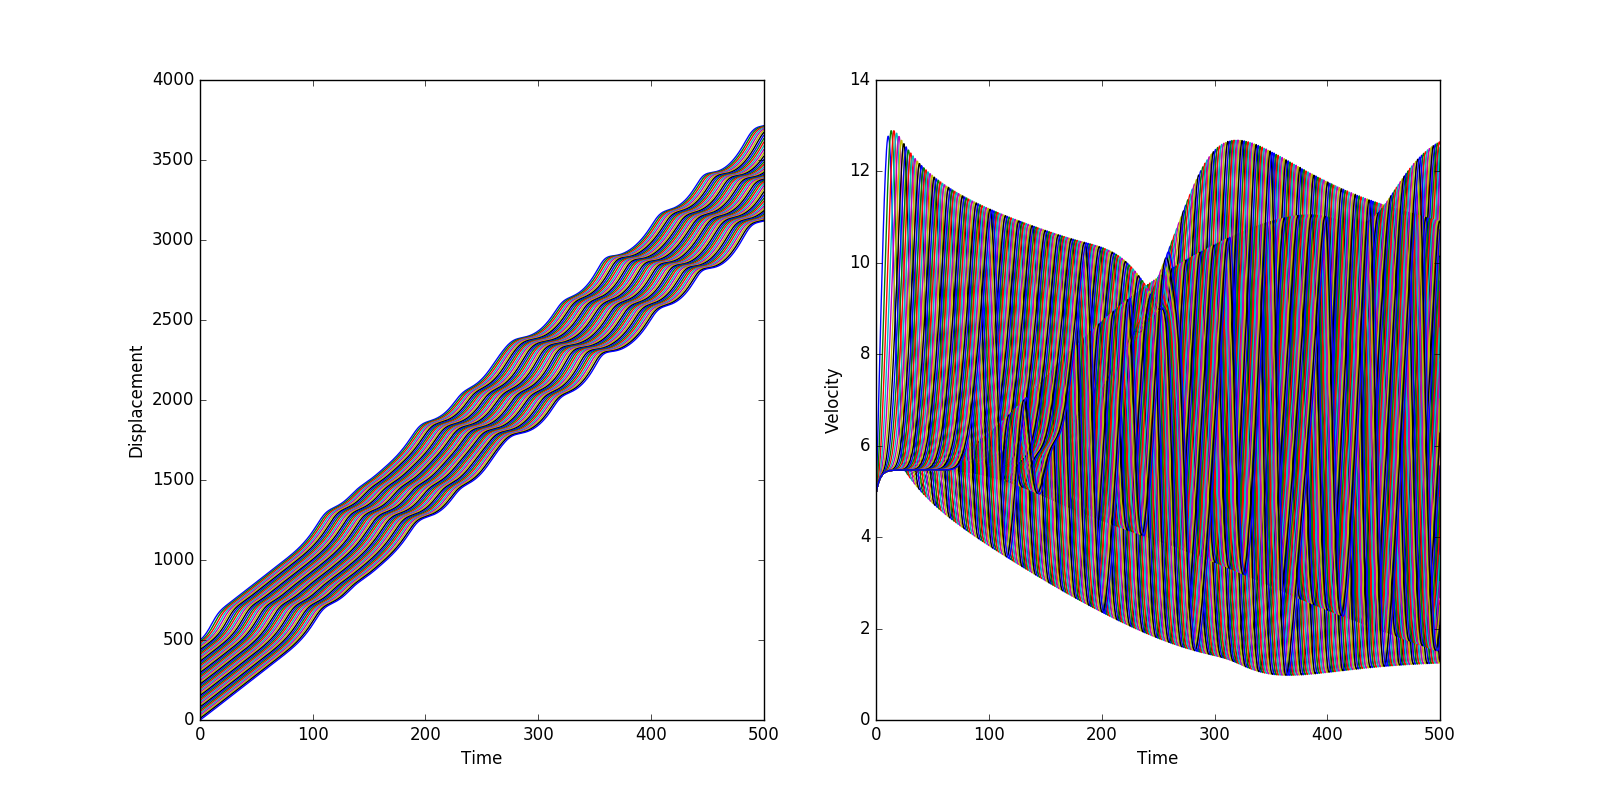
\includegraphics[width=0.95\textwidth]{maximise_distance.png}}
  \caption{System of IDM cars on a circular track optimizing for maximum distance traveled. The more aggressive driving of the cars results in wave formation.}
\end{figure}

\begin{figure}[H]
  \centering
  \fbox{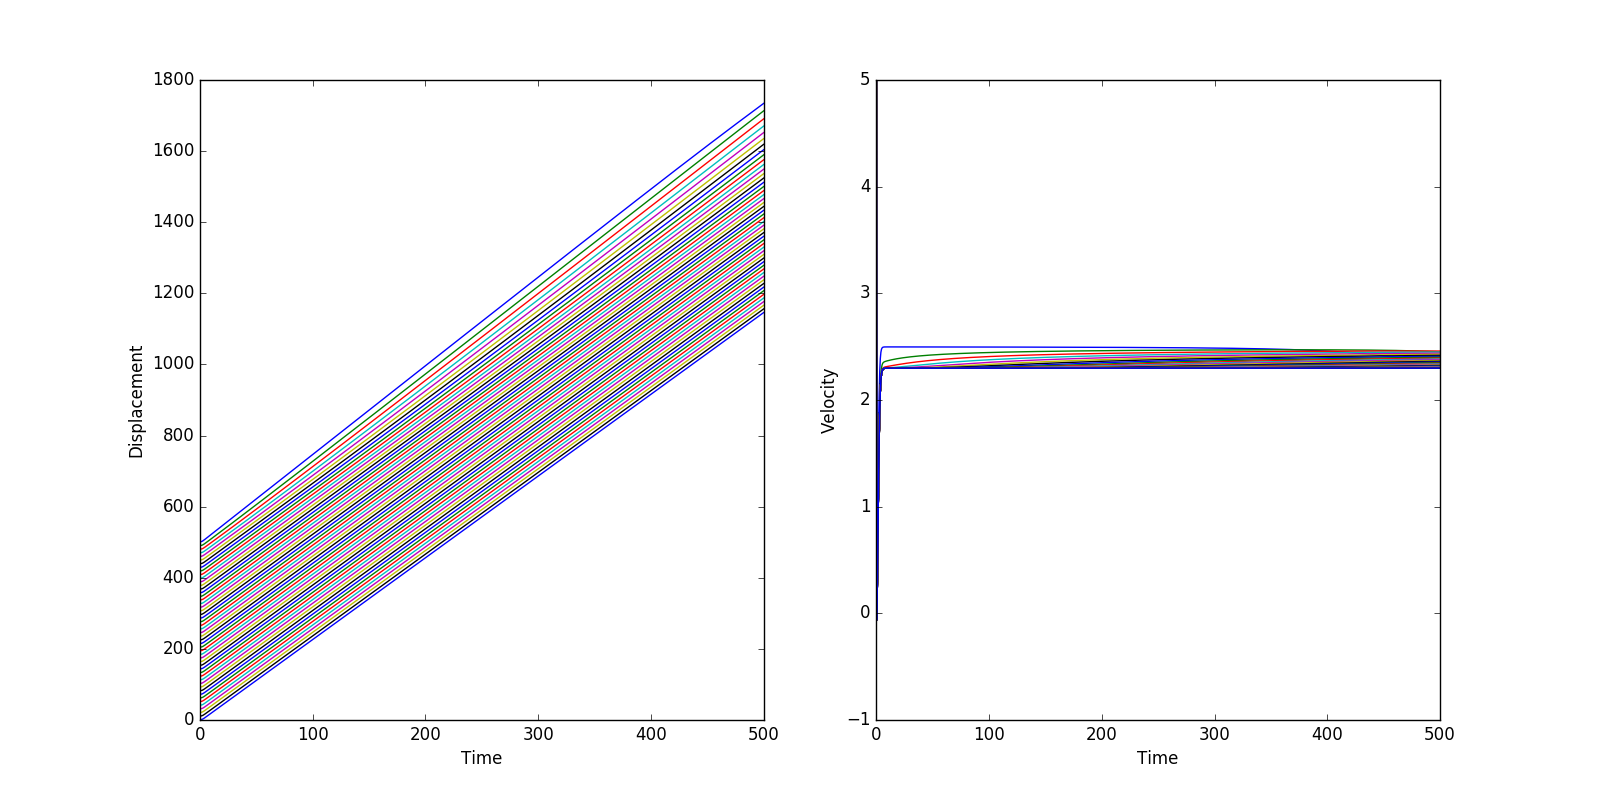
\includegraphics[width=0.95\textwidth]{optimise_comfort.png}}
  \caption{System of IDM cars on a circular track optimizing for maximum 'comfort' (minimum jerk). As one might expect, they choose to go rather slowly and thereby achieve a very stable velocity.}
\end{figure}

\section{Stability and Error Comparison of a Variety of Numerical Integration Schemes}
Because there is no analytical solution given for our highly-nonlinear problem, to analyze the error of our numerical integration schemes, we compared to the python \texttt{odeint} solver function. For large enough time steps, this shows us error decreasing on a log scale for each of our higher order methods. However, for small time steps, the `error` for 4th and 5th order methods converges, as the \texttt{odeint} solver presumably decides that 4th order is sufficiently accurate at these time steps and stops using higher order methods.\\
\begin{figure}
  \centering
  \fbox{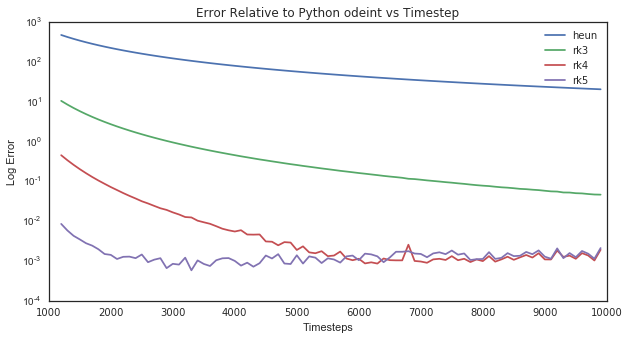
\includegraphics[width=0.95\textwidth]{error.png}}
  \caption{Error to odeint decreases with accuracy of finite differencing methods.}
\end{figure}
\paragraph{}For our purposes, we desired to use higher order methods such that we could use larger timesteps and hopefully decrease running time of our programs while still maintaining stability in the differential equation systems. To display the effectiveness of these higher order methods, we ran one of our simple models for a variety of time steps over the same total time with the different solvers and noted the number of time steps at which each method stabilized. We notice here that we don't see an additional benefit from using RK5, which in this case we suspect is because the extremely complicated coefficients are contributing to existing numerical overflow issues.\\
\begin{table}[H]
\centering
\caption{Timesteps for Stability with T=500s}
\label{my-label}
\begin{tabular}{lc}
 Method &  Minimum Timesteps for Stability\\ \hline
 Heun's Method & 325 \\
 Runge-Kutta 3 &  275\\
 Runge-Kutta 4 &  250\\
 Runge-Kutta 5 & 250
\end{tabular}
\end{table}

\section{String Stability of Traffic Systems to Perturbation}

The concept of string stability refers to whether a perturbation to the beginning of the system will result in a wave that dissipates or is enhanced as it propagates through the system. As we have seen in previous experiments that the IDM models are excellent for adjusting to and dissipating traffic perturbations, we expect them to be string stable and indeed they are.

\begin{figure}[H]
  \centering
  \fbox{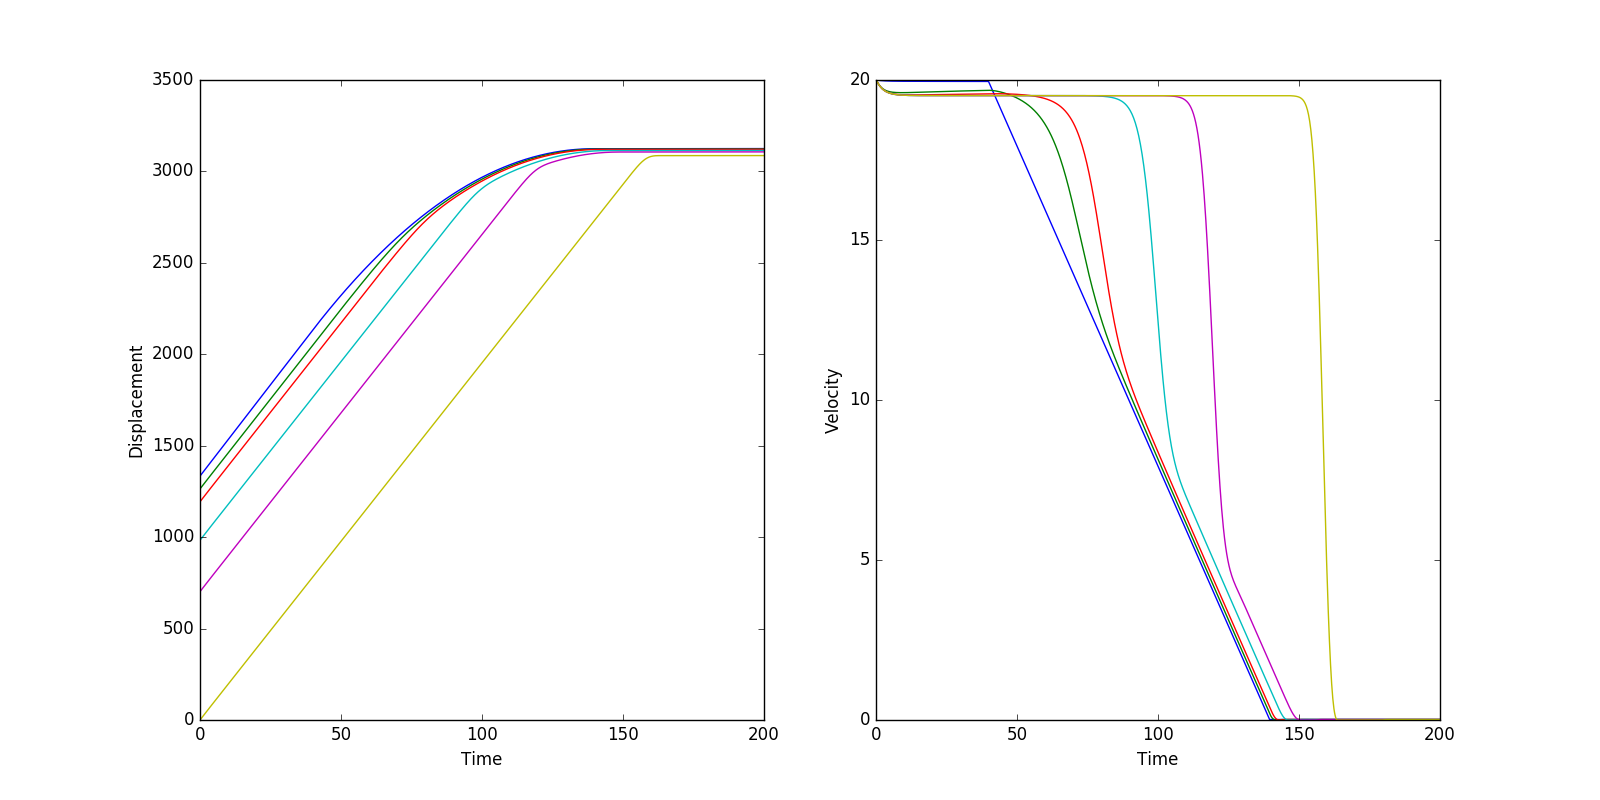
\includegraphics[width=0.95\textwidth]{displacement_and_velocity_plot_model0_ss.png}}
  \caption{Plot of cars 1,2,3,6,10, and 20 for IDM. String stable.}
\end{figure}

For HDM models, the presence or lack thereof of string stability depends on a number of parameters: number of leading cars being considered, time step ($\Delta t$), and reaction time ($T_r$). In general, string stability increases with number of leading cars being considered, although the marginal contribution of each car decreases to the point where there is not much additional benefit beyond 5 cars. String stability is inversely related to time step and reaction time, although reaction time has a greater effect. Below, we show two plots for parameters where the HDM system is string stable and string unstable.

\begin{figure}[H]
  \centering
  \fbox{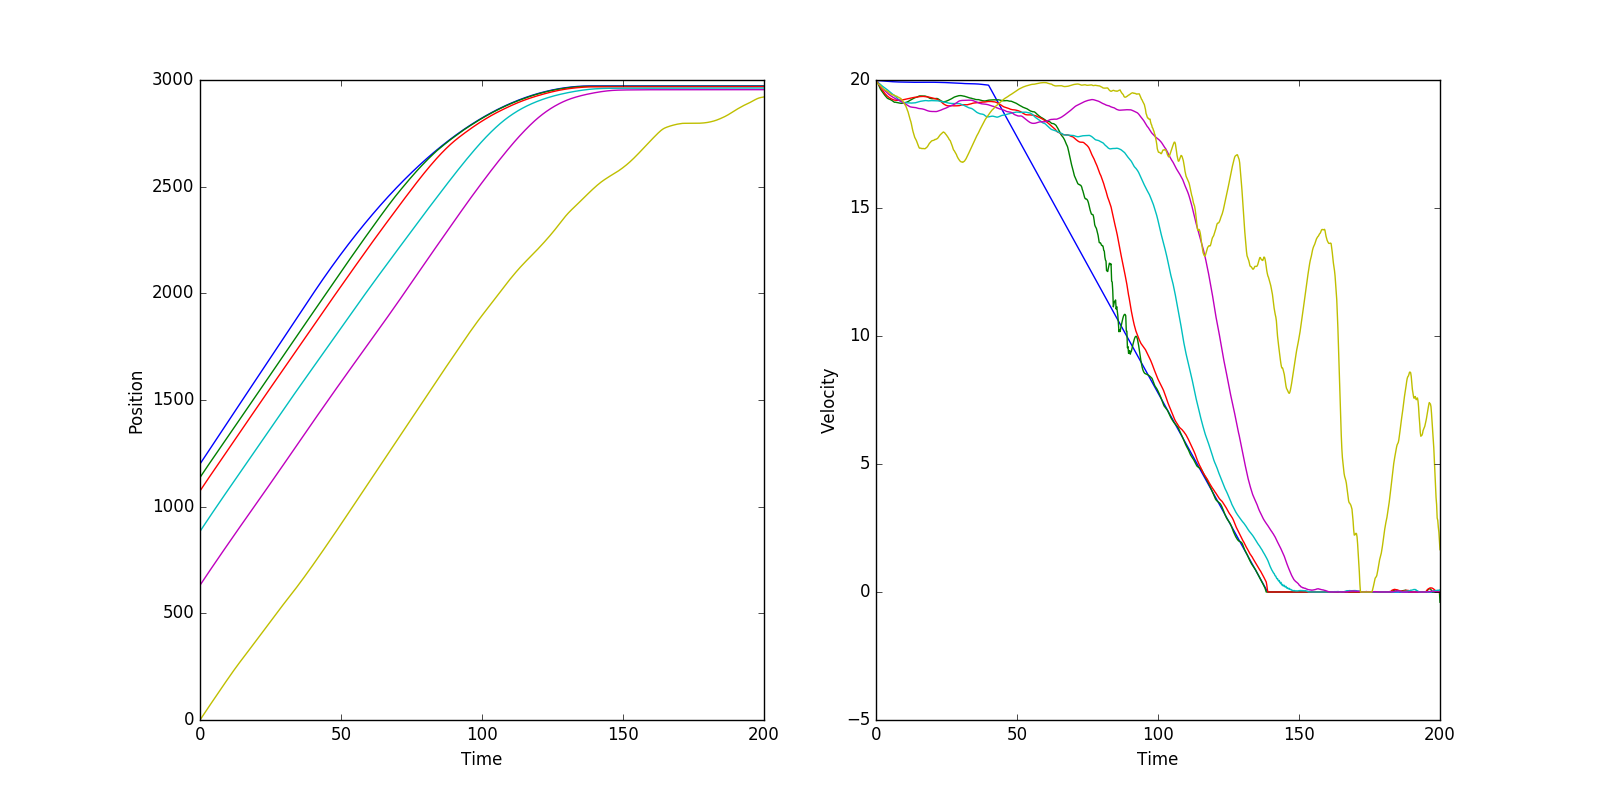
\includegraphics[width=0.95\textwidth]{HDM_anticipate_2_ss_1000_unstable.png}}
  \caption{Plot of cars 1,2,3,6,10, and 20 for HDM with two car lookahead. We see that for parameters $T_r$ = .6 and $\Delta t$ = .2, the system is string unstable, as evidenced by the large wave in car 20's velocity.}
\end{figure}

\begin{figure}[H]
  \centering
  \fbox{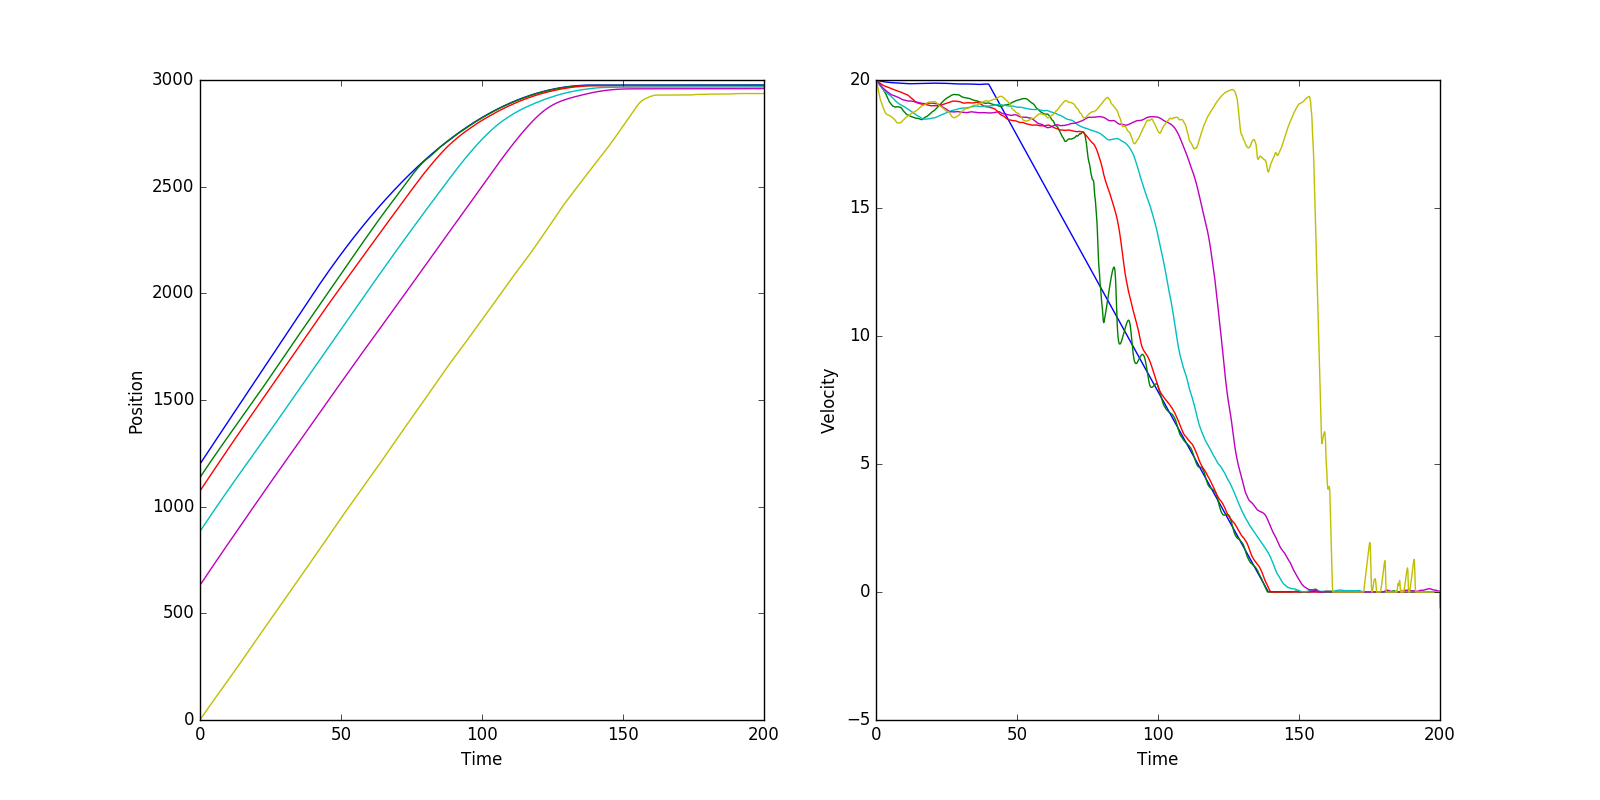
\includegraphics[width=0.95\textwidth]{HDM_anticipate_13002_ss_stable.png}}
  \caption{Plot of cars 1,2,3,6,10, and 20 with two car lookahead. We see that for parameters $T_r$ = .2 and $\Delta t$ = .15, the system is string stable.}
\end{figure}

\section{Optimization of Traffic Systems}
\paragraph{}We set up a number of optimization programs to attempt to search for the optimal values of some of the many parameters for the system as a whole and for individual drivers for a number of cost functions, including maximizing displacement and maximizing comfort (minimizing jerk). The initial trials for these systems were run on IDM models, and the results are largely what one would suspect. When attempting to maximize total displacement, the cars drive quickly and close together, resulting in the creation of traffic waves in the system. When attempting to minimize jerk, the cars drive much more conservatively, as one would expect, never coming within the range of another car that would cause them to change acceleration. \\
\textbf{RESULTS HERE}
\paragraph{}We then attempted to optimize behavior for a single driver and were interested to see what implications this would have for the system as a whole. However, the following behaviors in the IDM are such that a single driver can tailgate and maximize target speed basically as much as we will allow without ever disrupting the rest of the system. Even when adding some stochasticity to the lead car, we were unable to see the rest of the system suffer from traffic waves due to the behavior of the second car, because that behavior would simply be quickly dissipated by the third car. In fact, it seems to be true generally of these systems that unless the aggressive driving behavior of a car causes other cars to collide behind it, the greater distance achieved by one car inevitably results in other cars also achieving a greater distance/average velocity. \\

\paragraph{}Next, we attempted to replicate these experiments with the more complicated Human Driver Model. However, due to the highly piecewise nature of the functions we are attempting to optimize over, we were unable to use traditional minimization solvers. Instead, we discretized the parameter space we were interested in exploring and searched for the set of parameters which would minimize our target cost function. \\
Again, we find that in general maximizing displacement for a single car leads to greater displacement for the rest of the system unless the driving behavior is so aggressive that it results in a crash. Given that we have seen that the Human Driver Model is more likely to propagate perturbations, we had expected that there might be in this model a penalty to other cars in greater volatility of velocity, i.e. a less pleasant ride, but this effect was also not observed in the data. We conclude that the model is largely insensitive to individual parameters in this context and that the structure of the model tends not to penalize aggressive driving unless a collision results.\\
\begin{figure}[H]
  \centering
  \fbox{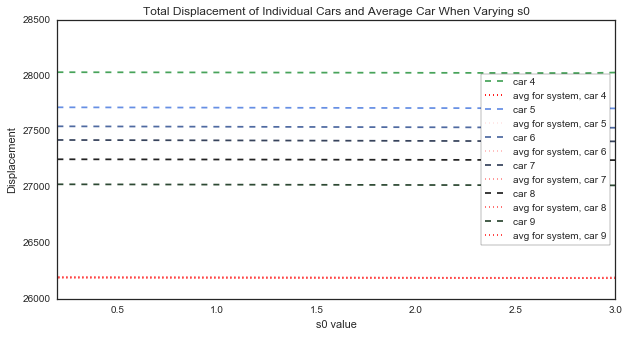
\includegraphics[width=0.95\textwidth]{optimize_s0_total.png}}
  \caption{Changing Safe Following Distance: Changes are minimal but overall distance increases for both the car in question and the system of cars with smaller distance.}
\end{figure}

\begin{figure}[H]
  \centering
  \fbox{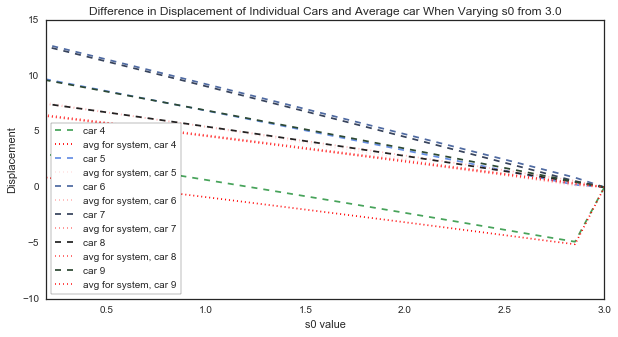
\includegraphics[width=0.95\textwidth]{optimize_s0.png}}
  \caption{Variation in Distance Traveled when Changing Safe Following Distance From Initial Value of 3.0}
\end{figure}

\begin{figure}[H]
  \centering
  \fbox{\includegraphics[width=0.95\textwidth]{optimize_t.png}}
  \caption{Changing Safe Following Time: Changes are minimal but overall distance increases for both the car in question and the system of cars with smaller.}
\end{figure}

\begin{figure}[H]
  \centering
  \fbox{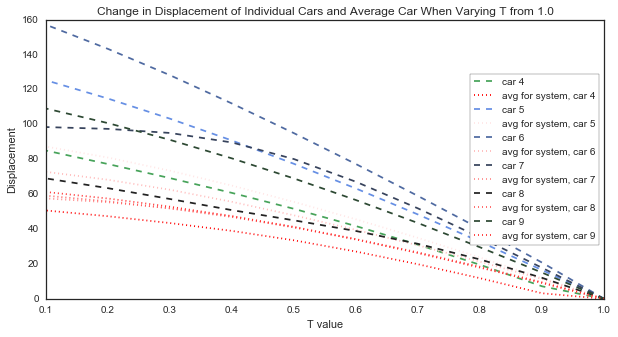
\includegraphics[width=0.95\textwidth]{optimize_t_change.png}}
  \caption{Variation in Distance Traveled when Changing Safe Following Time From Initial Value of 1.0}
\end{figure}

\section{TODO}
fuck this to do list, we've done enough. \\
develop a cost function for emissions/energy usage and optimize over that \\
can we find the parameters that will cause a phantom traffic jam?


\section{Discussion}

\section{Conclusion}



% Your references go at the end of the main text, and before the
% figures.  For this document we've used BibTeX, the .bib file
% scibib.bib, and the .bst file Science.bst.  The package scicite.sty
% was included to format the reference numbers according to *Science*
% style.
\newpage

\bibliography{bibliography}
\bibliographystyle{ieeetr}



\end{document}




















